\documentclass[a4paper,12pt]{article}
\usepackage[utf8]{inputenc}
\usepackage{microtype}
\usepackage{libertine}
\usepackage[libertine]{newtxmath}
\usepackage[scaled=.95]{inconsolata}
\usepackage[usenames,dvipsnames]{xcolor}
\definecolor{darkblue}{rgb}{0.0,0.0,0.55}
\usepackage{setspace}
\usepackage[top=2cm,bottom=2cm,left=2cm,right=2cm]{geometry}
\usepackage[backref,pagebackref]{hyperref}
\usepackage{graphicx}
\usepackage{float}
\usepackage{mathtools}
\usepackage{caption}
\usepackage[UKenglish]{babel}
\usepackage[UKenglish]{isodate}
\cleanlookdateon
\usepackage[authoryear]{natbib}
\usepackage{babelbib}
\exhyphenpenalty=1000
\hyphenpenalty=1000
\widowpenalty=1000
\clubpenalty=1000
\renewcommand*{\backref}[1]{}
\renewcommand*{\backrefalt}[4]{%
	\ifcase #1 (Not cited.)%
	\or        Cited on page~#2.%
	\else      Cited on pages~#2.%
	\fi}
\renewcommand{\backreftwosep}{ and~}
\renewcommand{\backreflastsep}{ and~}
\urlstyle{same}  % don't use monospace font for urls
\setcitestyle{aysep={}} 
\usepackage{etoolbox}
\makeatletter
\patchcmd{\NAT@citex}
	  {\@citea\NAT@hyper@{%
		 \NAT@nmfmt{\NAT@nm}%
		 \hyper@natlinkbreak{\NAT@aysep\NAT@spacechar}{\@citeb\@extra@b@citeb}%
		 \NAT@date}}
	  {\@citea\NAT@nmfmt{\NAT@nm}%
	   \NAT@aysep\NAT@spacechar\NAT@hyper@{\NAT@date}}{}{}
	\patchcmd{\NAT@citex}
	  {\@citea\NAT@hyper@{%
		 \NAT@nmfmt{\NAT@nm}%
		 \hyper@natlinkbreak{\NAT@spacechar\NAT@@open\if*#1*\else#1\NAT@spacechar\fi}%
		   {\@citeb\@extra@b@citeb}%
		 \NAT@date}}
	  {\@citea\NAT@nmfmt{\NAT@nm}%
	   \NAT@spacechar\NAT@@open\if*#1*\else#1\NAT@spacechar\fi\NAT@hyper@{\NAT@date}}
	  {}{}
\makeatother
\hypersetup{pdftitle={Beasts of Prey or Rational Animals? Private Governance in Brazil's Jogo do Bicho},
	pdfauthor={Danilo Freire},
	pdfborder={0 0 0},
	breaklinks=true,
	linkcolor=Mahogany,
	citecolor=Mahogany,
	urlcolor=darkblue,
	colorlinks=true}

\doublespacing

\title{\textbf{Beasts of Prey or Rational Animals?\\ Private Governance in Brazil's \textit{Jogo do Bicho}}}

\author{Danilo Freire\thanks{Postdoctoral Research Associate, Political Theory Project, Brown University, 8 Fones Alley, Providence, RI 02912, \href{mailto:danilofreire@brown.edu}{\texttt{danilofreire@brown.edu}}, \href{http://danilofreire.com}{\texttt{http://danilofreire.com}}. I would like to thank Toke Aidt, Paulo Roberto Araujo, Jose Bolaños, Diogo Costa, Guilherme Duarte, Robert McDonnell, David Skarbek, Graham Denyer Willis, the participants of academic seminars at King's College London, the University of Cambridge and the Prometheus Institut in Berlin, the editors of Latin American Perspectives, and four reviewers for their valuable comments. I gratefully acknowledge the financial support of the National Council for Scientific and Technological Development.}
}

\date{\today}

\begin{document}
\maketitle
\begin{abstract}
\noindent
This article presents a rational choice account of Brazil's \textit{jogo do bicho} (`animal game'), possibly the largest illegal lottery game in the world. Over 120 years, the \textit{jogo do bicho} has grown from a local raffle to a multimillion-dollar business, and it has played a major role in Brazil's cultural and political life. My analysis of the \textit{jogo do bicho} has three goals. First, I examine the mechanisms that fostered the lottery's notable growth outside of the boundaries of Brazilian law. Second, I investigate how the animal game financiers combine costly signals and selective incentives to induce cooperation from members of community. Lastly, I discuss the relationship between the lottery sponsors and Brazilian representatives, particularly how the \textit{bicheiros} exploit the fragmentation of the Brazilian political system to advance their long-term interests. 

 \vspace{.5cm}
 \noindent
 \textbf{Keywords}: Brazil; criminal organisations; corruption; \textit{jogo do bicho}; private governance
  
 \vspace{.25cm}
 \noindent
 \textbf{JEL Classification Codes}: D72, K42, Z00
\end{abstract}

\newpage

\section{Introduction}%
\label{sec:intro}

In 1892, Baron João Batista de Viana Drummond came up with a new idea to fund his cash-strapped zoo. Situated in a quiet neighbourhood in the north of Rio de Janeiro, the \textit{Jardim Zoológico}, or Zoological Garden, hosted a variety of exotic species and offered breath-taking views of the city. But it lacked visitors. An experienced businessman, Drummond realised the zoo would have to provide other kinds of entertainment to keep itself afloat. One of his plans seemed particularly promising: a lottery raffle.

The rules were straightforward. In the morning, the Baron would choose one animal from a list of 25 beasts and put its picture inside a wooden box at the zoo's entrance. Visitors who wanted to join the raffle received a ticket bearing the stamp of one of those 25 animals.\footnote{At first, the zoo staff distributed the tickets at random, but they soon allowed participants to choose the animals they preferred. This small change made the game considerably more appealing as it introduced an element of divination to the \textit{jogo} \citep[71--74]{da1999aguias}.} The lucky winner would take home a prize worth 20 times the ticket price, an amount higher than a carpenter's monthly wage \citep[542]{chazkel2007beyond}. The Baron called the lottery the \textit{jogo do bicho}, or the animal game, and it was well-received by the public. Eager to capitalise on that initial success, Drummond stated that visitors could buy tickets not only at the zoo, but also in many stores across Rio de Janeiro. What was once a small raffle soon became a large gambling market of its own. 

A \textit{jogo do bicho} craze swept the whole city after independent sellers entered the marketplace. A network of street bookmakers, called \textit{bicheiros}, made the lottery available in every part of Rio by scalping tickets or promoting their own versions of the numbers game \citep[37]{chazkel2011laws}. The lottery became so widespread that Olavo Bilac, a major literary figure in nineteenth-century Brazil, summarised the situation as follows: `Today $[1985]$ in Rio de Janeiro, the game is everything. $[\dots]$  Nobody works! Everybody plays' \citep[43]{pacheco1957antologia}.\footnote{Unless otherwise noted, all translations from the Portuguese are my own.} 

But this tolerant state of affairs did not last. Civil servants and police officers criminalised the \textit{jogo do bicho} on the grounds of `public safety', and in the late 1890s they launched a country-wide campaign against the lottery \citep{benatte2002jogos}. The campaign extended for several decades and received considerable support from the \textit{Companhia das Loterias Nacionaes do Brazil}, the National Lottery Company, a public-private partnership founded four years after, and perhaps motivated by, the creation of the animal game \citep[82]{da1999aguias}. The Brazilian government officially banned the \textit{jogo do bicho} in 1941 and it remains illegal until this day.  
 
Yet the game has survived. The \textit{jogo do bicho} has outlasted more than 30 Brazilian presidents and thrived under both military regimes and democratic governments \citep{jupiara2015poroes}. But more than a act of civic disobedience, the \textit{jogo do bicho} is a very successful capitalist enterprise \citep{labronici2014sorteio, magalhaes2005ganhou}. A recent study by Fundação Getúlio Vargas, a Brazilian think tank, affirmed that the \textit{jogo do bicho} earns from BRL 1.3 to BRL 2.8 billion per year (USD 400 to USD 850 million), making it the largest clandestine gambling game in the world.\footnote{See \href{https://www.huffpostbrasil.com/2015/12/07/legalizacao-jogos-brasil_n_8737212.html}{\texttt{https://www.huffpostbrasil.com/2015/12/07/legalizacao-jogos-brasil\_n\_8737212.html}} (in Portuguese). Access: August 2018.} \citet[171]{schneider1996brazil} estimated that in the 1990s, the game furnished about 50,000 jobs in the Rio de Janeiro city alone, almost the same number of employees that the oil giant Petrobras had in 2011 \citep{exame2013petrobras}.\footnote{In 1966, Time Magazine wrote that the \textit{jogo do bicho} was `the largest single industry in Latin America' and employed about 1\% of the total Brazilian workforce. See \href{http://content.time.com/time/magazine/article/0,9171,842527-1,00.html}{\texttt{http://content.time.com/time/magazine/article/0,9171,842527-1,00.html}}. Access: August 2018.}

In this article I offer a rational choice interpretation of the \textit{jogo do bicho}. More specifically, I use an array of bibliographical sources to show how the game operators, called \textit{bicheiros}, have developed unique strategies to solve collective action problems and maximise their political strategies. This does not mean that their tactics are morally defensible; \textit{bicheiros} regularly employ intimidation and corruption to achieve their goals. Nevertheless, I argue here that such strategies are effective, and while they seem counter-intuitive, they do address the long-term needs of the \textit{jogo do bicho} financiers. 

Like any business manager, \textit{bicheiros} have to run their firm with low costs to increase profits. However, the fact that the \textit{jogo do bicho} is clandestine imposes additional difficulties for its operation. In particular,  \textit{bicheiros} face two main challenges to keep the lottery running. First, they need to gather public support so that gamblers are not discouraged to engage in the lottery despite it being illegal. Second, \textit{bicheiros} also have to ensure that the state repression is not prohibitively costly to their business, otherwise they would be better off by shutting it down. I argue below that the \textit{bicheiros} have succeeded in both by using carefully-designed reputation strategies and employing costly signals to the communities they serve. 

I use the case of Rio de Janeiro to illustrate how the \textit{jogo do bicho} has overcome the obstacles to its expansion. Rio is a particularly interesting case because in no other part of Brazil the game financiers established such an effective patronage network. \textit{Bicheiros} have sponsored political campaigns, financed cultural activities and football teams, and sometimes even run in local elections themselves. I discuss the ways by which the \textit{bicheiros} have exploited fragilities of the Brazilian political system to their advantage and how those practices have weakened Brazilian democracy.   

My analysis discusses three strands of academic literature. First, this work contributes to the scholarship on extra-legal institutions, mainly to the literature on collective action within criminal organisations. For instance, \citet{gambetta1996sicilian} examines the strategies used by the Sicilian Mafia to settle disputes among their members and enforce rules in the areas they exercise control. \citet{leeson2009invisible,leeson2010pirational} affirms that pirate groups employed hard-to-fake signals to increase the profitability of their operations. \citet{skarbek2011governance,skarbek2012prison,skarbek2014social}, in turn, highlights the role of written and implicit norms in mitigating rent-seeking and coordinating productive activities in California prison gangs. I argue that \textit{bicheiros} have employed reputation strategies and provided club goods to enforce private contracts and foster trust in the community. 

Second, this work relates to the literature on signalling theory and asymmetric information \citep[e.g.,][]{akerlof1970market,spence1973job}. I provide evidence that \textit{bicheiros} were aware of their social stigma, and as a response they devised signalling strategies to convey reliable information and reduce the uncertainty associated with clandestine markets. Their main tool to increase credibility was costly signalling \citep{gambetta2009codes,kimbrough2015commitment, schelling1960strategy}. \textit{Bicheiros} believed that by sacrificing their immediate interests they could gain a reputation of honesty that would benefit them in the long run.  

Lastly, this work connects to the literature on state capture, which is one of the most important topics in public choice theory \citep{rose1978corruption,shleifer2002grabbing,tollison1982rent}. More specifically, I use the Brazilian case to illustrate how politicians and civil servants can be co-opted by criminal groups and produce bad social outcomes. \citet{queiroz1992carnaval} explored why \textit{bicheiros} turned into patrons of the Carnival's samba schools and affirmed that this influence gave them leverage over political authorities. \citet{misse2007illegal} investigated the links between bicheiros and police officers, and suggested that the illegal lottery had been the main cause of police corruption in Rio de Janeiro until the 1970s. In a similar vein, \citet{jupiara2015poroes} analyse the relationship between the \textit{jogo do bicho} and the military regime in Brazil (1964--1985). I supplement this literature by highlighting how asymmetrical information, agency dilemmas, and rent-seeking behaviour offer convincing explanations to the issues presented above. Although those concepts have a long tradition in public choice, scholars have not applied those ideas thus far to understand the dynamics of the \textit{jogo do bicho}. By doing so, I integrate seemingly contradictory historical facts into a single narrative that connects micro-level decisions to macro-level outcomes. 

\section{An Overview of the \textit{Jogo do Bicho}}%
\label{sec:overview}

\subsection{Historical Background: How the \textit{Bicheiros} Avoided Extinction}%
\label{sub:historical_background}

The late nineteenth-century Brazil had four characteristics that explain the emergence of the \textit{jogo do bicho}. They are: 1) a growing urban population excluded from the formal labour market; 2) an inflow of immigrants whose extended family networks helped them engage in trade; 3) an expansion of the monetary supply in the first years of the republic (1880s--1890s); and 4) a judicial system that, albeit repressive, had only imperfect law enforcement. I discuss each of these elements below.

I start with the impact of urban poverty on the animal game. Brazil abolished slavery in the late 1880s, a period in which the country was rapidly urbanising. Brazil's growing cities offered new occupations for former slaves who desired to move away from their former masters \citep{andrews1991blacks, skidmore1993black}. Increasing numbers of Asian and European immigrants joined the freed slaves and moved to the cities soon after they arrived in Brazil \citep{hall1969origins, lesser2013immigration}. However, the hopes of the African-Brazilians and the new foreign settlers would soon be frustrated by a series of economic downturns. The Brazilian labour market suffered a severe contraction in the wake of the \textit{Encilhamento} financial crisis of 1891, and the economic instability aggravated the already difficult conditions of the working classes \citep{topik2014political, triner2005baring}.

In that regard, large swathes of the urban population turned to the informal economy. As \citet[115]{chazkel2011laws} observes, there were few occupations available to lower-class women and foreigners in the 1890s, and a large number of poor workers became street vendors. The profession requires little technical skills and has low barriers of entry, but it can be very profitable if for whatever reason there is a strong demand for particular product. The \textit{jogo do bicho} was one of those products that offered a high rate of return. The game was simple to operate and that simplicity attracted more people willing to try their luck. As the game gained a following in Brazil's First Republic, it comprised an important share of the extra-legal economy in Rio de Janeiro.

Immigration also influenced the \textit{jogo do bicho} via social ties. Most foreigners who moved to Brazil came from countries, such as Portugal, Spain or Italy, where extended families were the basic form of social organisation \citep{lobo2001imigraccao, trento1989outro}. Family and neighbourhood networks created incentives for immigrants to establish trade relations and enforce cooperation through community responsibility systems \citep{roth2014prison}. Because of these particular social characteristics, in the 1890s foreigners were over-represented in the Brazilian trade in general \citep{mattos1991vadios, oliveira2001brasil} and in the \textit{jogo do bicho} in particular \citep{magalhaes2005ganhou, villar2008contravencao}. Although kinship bonds became less relevant over time, these links offered an important element of social cohesion in the \textit{jogo do bicho}'s formative years.

Next is the impact of expanded monetary supply. The abolition of slavery and the growing industrialisation of Brazil increased the amount of capital available in the country \citep{franco1987reformas, schulz2008financial}. Moreover, the 1888 Banking Act gave extra liquidity to local financial markets, what made credit more widely available in cities like São Paulo and Rio de Janeiro. Individuals received a temporary boost in personal income, a part of which they spent on leisure activities such as the \textit{jogo do bicho}. Moreover, the lottery attracted new entrants as it became more profitable, and in only a few years similar versions of the animal game were available throughout Brazil \citep[79]{da1999aguias}.  

The last necessary condition for the emergence of the \textit{jogo do bicho} is weak law enforcement. \citet[69--100]{chazkel2011laws} notes that until the 1940s, police district chiefs operated within a large margin of discretion, so official repression against bookmakers was notably inconsistent. In the early years of \textit{jogo do bicho}, lottery `bankers' were allowed to operate virtually free from police interference, what surely collaborated to the game's rapid initial expansion \citep[544]{chazkel2007beyond}. Prosecution against the \textit{bicheiros} hardened in 1917 after the promulgation of the Civil Code, and in 1941 the animal game was banned.\footnote{See \href{http://www.planalto.gov.br/ccivil_03/decreto-lei/Del3688.htm}{\texttt{http://www.planalto.gov.br/ccivil\_03/decreto-lei/Del3688.htm}} (in Portuguese). Access: September 2017.} Five years later, the federal government declared that all games of chance were illegal in Brazil.\footnote{The 1946 decree stated that gambling was `harmful to morality and the good customs', hence `[\dots] the repression against games of chance [was] an imperative of the universal consciousness'. The text can be read at \href{http://www.planalto.gov.br/ccivil_03/decreto-lei/Del9215.htm}{\texttt{http://www.planalto.gov.br/ccivil\_03/decreto-lei/Del9215.htm}} (in Portuguese). Access: September 2018.} Recent estimations show that the prohibition of the \textit{jogo do bicho} have prevented the state from earning BRL 15 to BRL 20 billion (USD 4.5 to USD 6 billion) per year in expected taxation revenues, aside from the subjective utility losses for players \citep{fsp2016legalizarbicho}.

Since the mid-twentieth century, the \textit{jogo do bicho} has been illegal but ubiquitous in Brazil. For all purposes, the \textit{jogo} remains criminalised, yet there is virtually no Brazilian city which does not have its local \textit{bicheiros}. The \textit{jogo} does not operate exclusively at the margins of the Brazilian law; it is clear that it consciously exploits and subsidises large sectors of the formal economy. I describe the animal game organisation structure and their impact in the Brazilian economy in further detail below.  

\subsection{A Hierarchical Organisational Structure}%
\label{sub:organisation}

The animal game operates with three levels of hierarchy. At the bottom level are the \textit{bicheiros}, those in charge of selling \textit{jogo do bicho} tickets \citep{chazkel2007beyond, da1999aguias}. \textit{Bicheiros} are the most visible part of the \textit{jogo do bicho}, and the name loosely describes all those involved in the lottery organisation. Yet their meaning in the \textit{jogo do bicho} structure is more particular and refers to street-level ticker sellers. The \textit{bicheiros}  usually build their vending stands inside the premises of a local shop, such as a small grocery store, and are recognisable by their chairs facing the street, stamps and blocks of paper \citep[259]{chazkel2011laws}. The street bookmakers usually work alone, but may employ up to 10 people depending on how busy their betting site is \citep[69]{labronici2014sorteio}.

The \textit{gerentes} (managers) oversee all \textit{jogo do bicho} stands in a given area. Their task is akin to that of a firm accountant. Gerentes control the cash flow between the \textit{bicheiros} and the bankers, manage the payroll of the employees, and provide financial information to the top members of the organisation. They also supervise individuals who carry menial tasks in the business, transfer money to other gambling branches and double-check the balance sheets of the betting sites \citetext{\citealp[71]{labronici2012paratodos}; \citealp[142]{misse2007illegal}}.

The \textit{banqueiros}, or the Portuguese for bankers, occupy the top position in the \textit{jogo do bicho} hierarchy. They comprise the small financial elite of the game. A 2012 report by the Brazilian Federal Police affirmed that 10 \textit{banqueiros} controlled the market throughout the country, and five of them were based in the state of Rio de Janeiro \citep{globo2012contraventores}. Apart from funding the game, the bankers provide support for the employees to undertake their activities. The \textit{banqueiros}' attributions include paying bribes to police personnel, bailing out sellers arrested by security forces, and offering judicial assistance to employees in case of legal persecution \citep[75]{labronici2012paratodos}.

The lottery bosses run their businesses from fortified houses in unknown locations, called the \textit{fortalezas} (`forts'). The first \textit{fortalezas} likely appeared in the 1950s, when the animal game was already well-established across the Brazilian territory. The period coincides with a time when the \textit{jogo do bicho} finances had become increasingly concentrated in fewer hands \citep[259]{chazkel2011laws}. Due to the growing scope of the \textit{jogo do bicho} economy, \textit{banqueiros} decided to move their operations away from the public to avoid police persecution and make coordination easier. 

\textit{Banqueiros} solve problems of internal cooperation by providing club goods \citep{buchanan1965economic} while simultaneously shunning cheaters through selective punishments \citep{bo2005cooperation, roth1978equilibrium}. The first club good offered to \textit{bicheiros} by their bosses is private security. As the game is illegal, street sellers cannot rely on official institutions to protect themselves. Thus, the game bankers have built an extensive network of gunmen and bribed police officers to protect their employees from other criminals \citetext{\citealp[48]{chinelli1993vazio}; \citealp[51]{labronici2012paratodos}}. `Zé' (Joe), a bicheiro interviewed by \citet[52]{labronici2012paratodos}, described eloquently the deterring effect of the \textit{jogo do bicho} informal security personnel:

\begin{quote}
 [\dots] bums are scared and they don't mess around with us; they think there's an officer nearby or something like that. Look at all this money here! [shows the interviewer a handful of cash] It's not ours [referring to street-corner bookmakers]. And if it's not ours, it's someone else's. When I worked in Penha\footnote{Penha is a low middle-class neighbourhood in the city of Rio de Janeiro.}, the owner of a pub close by always asked me to stay at the front door of his pub. People know that bums are afraid of \textit{bicheiros}.
\end{quote}

But the \textit{banqueiros} do not use violence only against other criminals. They often employ violent methods against competitors and their own staff, too. \citet{jupiara2015poroes} argue that Ailton Guimarães Jorge, a former Army officer, tortured and murdered rival lottery bosses in the late 1970s. One of his former allies, Army Colonel Paulo Malhães, told to the Rio de Janeiro State Truth Commission that Guimarães `went on a rampage' to consolidate his power \citep{belem2015guimaraes}. Castor de Andrade, Rio's most influential animal game banker, also employed similar methods to run his business. Andrade kept an armed bodyguard of 23 men and allegedly murdered a number of competitors. In a famous case, Andrade shot Euclides Ponar, an old \textit{jogo do bicho} boss known as `Grey-Headed Chinese' (\textit{China Cabe\c{c}a Branca}) after Ponar denounced a fraud in lottery draws in 1976. Andrade was likely involved in other assassination plots in the 1990s  \citep{globo2017castor}. 

Despite these serious events, killings are rare in the animal game. Since the lottery bosses can credibly indicate that violence is a low-cost option for them, the mere threat of punishment is enough to discourage defectors. This is a good strategy for the \textit{banqueiros}. The fact that they had committed violent crimes in the past reduces the need to commit them in the present, as and a result the bosses can spend less money on security and increase profits. As it happens in many traditional markets, if a group is able to form a cartel, they can increase the price of their services without fearing immediate competition. The same logic is valid for the \textit{jogo do bicho}, although through unconventional means.  

The threat of violence is not the only tool the \textit{bicheiros} have at their disposal. They balance the use of violence with financial benefits to low-rank members of the organisation. For instance, street \textit{bicheiros} keep all tips they receive from players, often have small expenses covered by their bosses, and may request interest-free loans to pay for healthcare treatment or other unexpected bills \citep{labronici2012paratodos}.

The most important financial mechanism implemented by bankers to help \textit{bicheiros} is the \textit{descarga}, loosely translated as `the unloading'. The descarga is the \textit{jogo do bicho}'s main hedging technique and its purpose is to insure small bookmakers against credit risk \citetext{\citealp[59]{labronici2012paratodos}; \citealp[178]{magalhaes2005ganhou}}. Booking agents are sometimes unable to honour expensive bets. The top prize in the animal game pays up to 4,000 times the amount invested, thus \textit{bicheiros} may have to raise thousands of Brazilian Reals in a single day to pay the lucky winners. To prevent the \textit{quebra da banca} (`bust of the bank'), \textit{bicheiros} and small bankers buy an insurance from wealthier financiers, who offer this service for a fee that ranges from 20\% to 25\% of the total selling amount \citep{fsp2006descarga}. The \textit{descarga} guarantees that small bookmakers will not have liquidity problems, thus permitting bookmakers to continue investing in the \textit{jogo do bicho}.

The \textit{descarga} has significantly changed the distribution of resources in the \textit{jogo do bicho}, and the richest bankers benefited the most from it. Simple probability dictates that a booking agent rarely pays the highest lottery prize, and yet the bankers receive a commission for \textit{every game} they hedge. Over time, there is a transfer of income from the bottom to the top of the animal game structure due to the fees. This accumulation of capital is one of the reasons why in the 1990s bankers started offering other types of entertainment such as slot machines and sports lotteries \citep{estado2006cacaniquel,globo2015cacaniquel,terra2011cacaniquel}. They simply had more capital to invest, and this eventually helped to compensate the downturn in the \textit{jogo do bicho} markets in the last years \citep{globo2017castor}. In sum, while the \textit{descarga} has made the game more resilient at the aggregated level, it increased profits for the richest financiers at the expense of small bookmakers.

This has brought broad consequences to the Brazilian illegal economy. As the number of slot machines increased in Brazil, the opportunity for criminals to use them for money laundering are higher as well. The scheme is easy to carry out. The owner of a slot machine issues a ticket with a winning prize, and the criminal declares the prize as his legitimate wealth. Then he can legally use that money for any purpose without raising suspicion from the authorities. The practice have become more widespread in the last decades, and in 2009 a Federal Police task force arrested about a dozen \textit{jogo do bicho} bosses involved in the so-called `the slot machine mafia', including relatives of Castor de Andrade \citep{estado2011cacaniquel}. In 2012, President Dilma Rousseff sanctioned a law that considered slot machines and the \textit{jogo do bicho} as money laundering \citep{agenciabrasil2012dilma}. 

Money from the \textit{jogo} also has other effects on the economy. Some of these effects are indirect. For instance, the \textit{jogo do bicho} gives a boost to the Brazilian economy by providing jobs for unskilled workers who cannot easily join the labour market. By doing so, the \textit{jogo} prevents some of poorest members of the Brazilian society from demanding more inclusive government policies, although they are the ones who would benefit the most from public assistance. Because of the income generated by the \textit{jogo do bicho}, poor workers are able to consume without resorting to government assistance, so state officials can spend a larger amount of public funds spent on other, probably wealthier, sectors of the population.

Another indirect economic effect of the \textit{jogo} is the rise in inequality. While formal workers can -- at least in theory -- demand higher compensations during a market upswing, the same is not true for the animal game employees. The threat of violence reduces the space for collective bargaining with the lottery bosses, and increasing profits at the top of the \textit{jogo do bicho} structure do not trickle down to higher salaries at the bottom. This is one of the reasons why the game bankers turned the game into an oligopoly: the use of violence guarantees not only that new entrants will not be allowed to join the market, but also that profits are concentrated in the hands of very few individuals.  

The \textit{jogo do bicho} market formation closely resembles what \citet{fligstein1996markets} calls `markets as politics', in which firms create institutions to restrain the competition and organise the labour force. At the formation of the lottery market, competition is fierce and incumbents an challengers are akin to social movements. They are constantly trying to convince others of the viability of their ideas. When markets stabilise, however, incumbents collude to impose their conditions of control to other players and to workers. In the case of the \textit{jogo}, this implies in a mix of financial incentives and violence threats carried by corrupt state agents or private bodyguards. 

A more difficult question is how the bankers elicit cooperation from \textit{external} members, such as gamblers, community leaders, or public officers. It is puzzling because \textit{bicheiros} do not use violence to induce individuals to play the lottery, nor have they ever clashed with the Brazilian government. Precisely because violence could shun off profits, \textit{bicheiros} devised other mechanisms to create a friendly environment for the illegal lottery. In the next section, I investigate two of them, costly signalling and reputation building. 

\section{Winning Hearts, Minds, and Pockets: Illegal Market Dynamics}%
\label{sub:pockets}

Evolutionary game theory \citep{axelrod1984evolution, axelrod1985achieving, smith1982evolution} and empirical case studies \citep{isaac1984divergent, ostrom1990governing} have both demonstrated that long-term cooperation is possible even in difficult situations. The main requirement for sustained cooperation is that players believe that future pay-offs will be higher than present ones. If that condition is true, fear of retaliation will induce individuals not to cheat. 

In theory, the same should also apply to illegal organisations. Yet in practice we see that criminal groups are generally short-term oriented, that is, they tend to discount the future more heavily that most people. This makes cooperative behaviour among criminal rather uncommon, and there is substantial evidence suggesting that illegal groups face serious collective action problems \citep[e.g.,][]{gambetta2009codes, leeson2010pirational, skarbek2011governance, skarbek2012prison, varese2001russian}. 

The \textit{jogo do bicho} is an exception to this rule. The game has been running for more than a century without considerable interruption, what attests that \textit{bicheiros} have managed to solve collective action issues in one way or another. Importantly, the \textit{jogo} involves moderately low levels of violence -- at least when compared to other illegal activities such as drug trafficking. Moreover, Brazilians widely consider the \textit{jogo do bicho} an honest lottery, and reports of cheating are surprisingly uncommon. The popular motto associated with the game testifies in its favour: `\textit{vale o escrito; ganhou, leva}', or `what is written is what counts; if you win it, you take it' \citep{magalhaes2005ganhou}. Here I analyse two means by which the \textit{bicheiros} elicit voluntary cooperation from gamblers and members of the community, costly signalling and reputation strategies. 

Signalling theory predicts that when someone cannot easily observe a characteristic she is interested in, she searches for signals that credibly conveys pieces of that required information. In the case of an illegal lottery, the main signal a gambler is looking for is \textit{honesty}, that is, that she has a fair chance of winning the game if she makes the right bet. 

Legal lotteries employ many techniques to show that this is the case. For instance, the Brazilian official lottery, run by the federal government, are regularly audited by the \textit{Controladoria Geral da União} (Comptroller General of Brazil), the \textit{Tribunal de Contas da União} (General Accounting Office), and by Ernst \& Young. The balls are measured and weighted every three months by the National Institute of Metrology, Quality and Technology (Inmetro), the Brazilian equivalent of United Kingdom's National Physical Laboratory or the American National Standards Institute.\footnote{See \href{http://noticias.uol.com.br/cotidiano/ultimas-noticias/2016/04/08/auditoria-dos-sorteios-da-caixa-e-confiavel-veja-como-e-o-processo.htm}{\texttt{https://bit.ly/2q3XnAV}} (in Portuguese). Access: December 2016.} A clandestine lottery, in contrast, cannot provide the same signals. Thus, the game providers need to assure gamblers that their business is honest although it is illegal. \textit{Bicheiros} addressed this issue using a traditional commercial practice: they invested on their reputations.   

The \textit{jogo do bicho} entrepreneurs have made considerable efforts to present themselves as honest brokers. The first trust-enhancing mechanism they have employed to foster external cooperation was the use of a \textit{fixed-multiplier formula} for pay-outs. It works as follows. If a player wins the lowest prize of the animal game, he or she receives 18 times his/her investment regardless of the size of the bet. Bigger prizes naturally offer higher returns; a lucky winner of the top prize wins up to 4,000 times the value of his/her bet \citetext{\citealp[89]{labronici2012paratodos}; \citealp[20]{magalhaes2005ganhou}}.

This stands in sharp contrast to the common practice of sharing a prize among winners. Lottery pay-outs demand high levels of interpersonal trust: players rely on unverifiable information about the total funds collected by the lottery, and they can never be sure whether the payments are evenly distributed. The fixed-multiplier formula alleviates such problems of adverse selection \citep{akerlof1970market, cohen2010testing, levin2001information}. As players and vendors known the prize value beforehand, the method provides consumers with complete information about their individual prizes while also binding the \textit{bicheiros} to a contract that can be easily enforced. This technique offers buyers a simple yet effective screening strategy that induces \textit{bicheiros} to provide honest information about the game \citep{spence1973job, stiglitz1981credit}.

\textit{Bicheiros} have addressed information asymmetries in another ways. Since the 1950s, when the \textit{jogo do bicho} bankers had moved their operations to the \textit{fortalezas}, the public could not oversee the lottery draws \citep[259]{chazkel2011laws}. This could lead to a decline in trust among buyers and vendors of lottery tickets and, as a result, to reduced profits. \textit{Bicheiros} have mitigated this problem with a two-pronged strategy. First, they started to utilise the winning numbers from the licit government-run lottery, the \textit{Loteria Federal}, instead of their own draws \citetext{\citealp[546]{chazkel2007beyond}; \citealp[89]{labronici2012paratodos}; \citealp[39-40]{mello1989historia}}. The federal lottery numbers are public information. The media broadcasts the draws on radio and TV, so any interested player can verify the selected numbers. The Loteria Federal is also audited by two independent state institutions, a private accounting firm, and voluntary members of the public; hence, \textit{bicheiros} can free ride on the lottery's long-standing reputation of credibility.

Second, they included representatives of all major \textit{jogo do bicho} bankers in every draw and independently publicise the game results. Certain \textit{bicheiros} went as far as publishing the numbers in Rio's newspapers. In the early twentieth century, some tabloids were entirely dedicated to the game \citep[60]{magalhaes2005ganhou}. Booking agents see this strategy as a credible signal from the game financiers, as providing contrasting information would indicate game manipulation. Moreover, collusion can also be spotted if the draws show repeated numbers or unusual patterns.

These efforts have proved popular with the game enthusiasts. Such mutual confidence reduces the potential for conflict in the game. As the public does not see the \textit{jogo do bicho} as violent or harmful, the stigma of repugnance associated with gambling becomes less pervasive. By reducing the possibilities of cheating and putting long-term interests first, the \textit{jogo do bicho} bankers have avoided the fate of other repugnant markets \citep[20]{da1999aguias}.

This ability to elicit cooperation from external actors caused the \textit{jogo do bicho} to last longer than collection action theories would anticipate. In that regard, the bankers' investment in costly signalling and reputation has largely paid off: the lottery's continuous profits are a proof of their success. With that continuous flow of income, \textit{banqueiros} were able to extend their influence well beyond the poor communities in which they operate. One of these areas is politics. 

\section{Tropical State Capture: \emph{Jogo do Bicho}, Samba and Politics}
\label{sec:capture}

The impact of the \emph{jogo do bicho} is not restricted to the Brazilian economy. Since the 1960s, \emph{bicheiros} have been the key sponsors of the country's most important cultural and social festivity, the Rio de Janeiro Carnival parade \citep{bezerra2009mecenato,cavalcanti2006carnaval,chinelli1993vazio,queiroz1992carnaval}. The \emph{jogo do bicho} accounts for such large share of the funding of the parade that a famous \emph{banqueiro} once remarked that `without the \emph{jogo do bicho} the Carnival would have ended' \citep{odia2016aniz}. Owing to that support, \emph{bicheiros} have established an extensive patronage network with samba schools and local politicians \citetext{\citealp[4641]{arguello2012criminalizaccao}; \citealp{congressoemfoco2007bicho}; \citealp{jornaldobrasil2011bicho}; \citealp[16]{misse2011crime}}. Although that network brings large material benefits to their members, the patronage system has created perverse incentives for government officials.

The \emph{jogo do bicho}'s clientelism is more evident in the state of Rio de Janeiro than in other parts of the country. Historical factors explain why this is the case. Firstly, Rio de Janeiro city was the capital of Brazil for almost 200 years; despite losing the position to Brasília in 1960, it remains one of the country's main cultural and financial centres. Secondly, \emph{jogo do bicho} operators had historical ties with popular movements, which they eventually exploited to their advantage. Thirdly, the emergence of state-sponsored Carnival parades created a window of opportunity for \emph{bicheiros} to expand their influence over public authorities, either via bribing or by funding political campaigns. In this regard, Rio provided a suitable environment for self-interested politicians, community leaders and animal game financiers to collaborate. These illegal networks are crucial to understand why samba and Carnival became constituent features of Brazil's national identity, and how the festival has contributed to Rio's high levels of state corruption.

\subsection{The `Medici of Samba': \emph{Bicheiros} as Patrons of Carnival}
\label{sub:patrons}

In 1930, opposition leader Getúlio Vargas led a bloodless coup d'état that brought Brazil's First Republic to an end. During his first presidency (1930--1945), Vargas promoted a radical shift in Brazilian politics by dismantling effectively federalism in favour of a powerful executive branch and an expanded federal bureaucracy \citep[e.g.][]{bethell2008politicsvargas,desouza1983estado,fausto1972revoluccao,fausto2014concise,skidmore1967politics}. In terms of ideology, Vargas's authoritarian-corporatist \emph{Estado Novo} (``New State'') promoted a politicised nationalism designed to transcend the regional aspects of Brazilian culture \citep{lauerhass1972getulio,nava1998lessons,williams2001culture}. Popular music, in turn, occupied an important place in Vargas's project of `brazilianing Brazil'. Created in the late 1920s in the shanty towns of Rio de Janeiro, modern samba embodied the idea of the multicultural, racially-tolerant country the government aspired to forge \citep{avelar2011brazilian,mccann2004hello,stockler2011samba,vassberg1969villa,vassberg1975villa}.

By the late 1930s, samba reached a unique position in Brazil's cultural identity. In a period when civil and political rights were limited \citep{de2001cidadania,duarte1993vicissitudes}, Vargas used samba as a means to incorporate ethnic minorities and the new urban classes into the Brazilian mainstream \citep[213]{chinelli1993vazio}. Patriotic sambas exalted the country's natural beauties and the figure of the `friendly, happy, cordial and industrious' mulatto\footnote{A mulatto is a person of mixed white and black ancestry. The etymology of the word is originally derogatory as it alludes to `mule' (Latin: \emph{mulus}), the infertile offspring of the male donkey and a female horse. However, in the 1930s the word loses its pejorative connotation in Brazil. Mainly due to the work of sociologist \citet{freyre1933casa}, the idea of a racial democracy becomes pervasive in the government discourse, and as a result the word gains a positive tone \citep[4]{reiter2009brazil}.} \citetext{\citealp[47]{dangelo2016samba}; \citealp[51]{vianna1995misterio}}. The institutionalisation of the Carnival parade in 1935, and the subsequent increases in public funding to the festival, cemented the relationship between politicians and samba groups \citep{almeida2017carnaval,cabral2016escolas,soihet1998subversao}.

However, the samba groups were not passive members in this process. Since the 1960s, the Rio Carnival expanded in scope and, stimulated by growing numbers of spectators, the parades became more elaborate \citetext{\citealp{cabral2016escolas}; \citealp[214]{chinelli1993vazio}; \citealp[240]{hertzman2013making}}. Unable to cope with the rising costs of the show, the `samba schools', which are large samba groups that compete in the Carnival, resorted to the \emph{jogo do bicho} financiers to fund their activities \citep{misse2007illegal}. This informal agreement between samba school organisers and wealthy \emph{bicheiros} remains effective to this day, and many of Rio's most famous samba schools are officially presided by high-profile members of the \emph{jogo do bicho} elite \citep{bezerra2009mecenato,cavalcanti2006carnaval,farias2013carnival,misse2011crime,queiroz1992carnaval}.

As I have mentioned in the previous section, the animal game at times faced opposition by the local population. The public often perceived the game as immoral and repugnant. Moreover, even after the bicho was well-established in Rio de Janeiro, the transition from a competitive betting market to an oligopoly involved the threat and often the use of physical violence against bookmakers who resisted the change \citetext{\citealp[143]{bezerra2009mecenato}, \citealp[52]{labronici2012paratodos}}. \emph{Bicheiros} were aware of the reputation costs their strategy entailed. They decided to finance samba schools hoping to win `the hearts and minds' of the population and attach a more positive image of the game among urban classes. Members of the \emph{jogo do bicho} had been involved in the Carnival since the early 1920s, but only as individuals who had a private interest in samba \citep[209]{chinelli1993vazio}. In 1984, a group of rich \emph{jogo do bicho} financiers founded collectively the LIESA (\emph{Liga Independente das Escolas de Samba}, Independent League of the Samba Schools), a civil association intended to direct and sponsor the Carnival parade in Rio de Janeiro. The LIESA marked a shift in the Carnival. For the first time, \emph{bicheiros} decided to act as a group rather than individuals. The organisation consolidated the power of \emph{bicheiros} over the parade and provided a formal mechanism to solve disputes among the samba school patrons \citetext{\citealp[43]{cavalcanti2006carnaval}; \citealp[171]{farias2013carnival}; \citealp[55]{labronici2012paratodos}}.

The funding of the samba schools had an indirect effect to the animal game. The patronage also reduced agent-principal problems within the \emph{jogo do bicho}. \emph{Bicheiros} donate to samba school to gather support of the communities, and by doing so they gain access to local information on their business. Clients who have a positive image of the \emph{bicheiro} may denounce fraudsters to their superiors, thus monitoring is cost-effective for animal game managers. Thus, street bookmakers have fewer incentives to cheat. In addition, street sellers are often recruited from the poor communities, so they tend to be immediate beneficiaries of \emph{bicheiros}'s donations \citep{bbc2012aniz}. Hence, funds donated to samba schools and other charities organisations help align the interests of different members of the \emph{jogo do bicho} organisation. The patronage can be interpreted as an illegal version of `profit-sharing', a mechanism which has induced effectively cooperative behaviour in both small and large corporations \citep{cahuc1997profit,fitzroy1987cooperation, kruse1992profit}.

The samba schools have profited from this association too. First, they have gained autonomy from the government. The samba schools do not need to rely exclusively on public funds to organise the parade, and money from the \emph{jogo do bicho} permitted the schools to act independently \citep[209]{chinelli1993vazio}. Second, the support of the \emph{jogo do bicho} has increased the political and social clout of the samba schools. In a country where the state is not present throughout the territory and human right abuses are frequent \citep{ahnen2003,odonnell1993state,pinheiro2000,pinheiro2001}, \emph{jogo do bicho} bankers, and more recently drug traffickers, have provided private governance to poor areas of Rio de Janeiro by enforcing property rights, mediating disputes, and preventing police abuse in the favelas \citep{arias2006dynamics,goldstein2013laughter,leeds1996cocaine}. In return for funds and protection from the \emph{bicheiros}, samba schools have served as intermediaries between the underworld and the political system. Although the \emph{banqueiros} are interested in weak law enforcement against the animal game, politicians have resorted to samba schools to contact \emph{bicheiros} and use their financial and electoral influence in the shanty towns \citep[17]{misse2011crime}. The samba schools, therefore, have increased their bargaining power in the political sphere and extended their reach within Rio's poor communities \citep[215]{chinelli1993vazio}.

\subsection{Political Support}
\label{sub:support}

If politicians were opposed to the \emph{jogo do bicho} in the early twentieth century, their relationship with the animal game bankers have become more ambivalent in the last decades. The collaboration between public authorities and \emph{bicheiros} gained prominence during the military dictatorship (1964--1985) \citetext{\citealp{gaspari2002ditadura}; \citealp{jupiara2015poroes}; \citealp[39]{zaluar2007democratizaccao}}. Given the absence of democratic checks and balances, paramilitaries and police forces colluded to repress potential dissidents of the regime and, frequently, to extort civilians \citep{gorender1999combate,magalhaes1997logica,misse2009acumulaccao,skidmore1990politics}. \emph{Bicheiros} saw the corruption of some members of the military as an opportunity. Wealthy \emph{jogo do bicho} bankers hired rogue police officers not only to work as security guards but to threaten eventual competitors in their regions of influence. The agreement between \emph{bicheiros} and corrupt members of the military was the ultimate responsible for the transformation of the \emph{jogo do bicho} into a `coercive oligopoly' \citep{jupiara2015poroes}. The support of the armed forces meant that new groups would be prohibited from entering the market and that the illegal lottery could operate undisturbed by the government.

The links between \emph{bicheiros} and the public authorities changed after Brazil became a democracy in 1985. In the military regime, government officials were mainly interested in bribes from the animal game. But in the democratic period, votes became a sought-after political resource. \emph{Bicheiros} are important in this sense as they have direct influence over a number of poor communities. Their patronage networks ensure that candidates supported by \emph{bicheiros} receive a substantial amount of votes from areas where campaigning is too difficult or too costly \citep[17]{misse2011crime}.

The Brazilian political system is particularly conductive to clientelistic practices. Brazil has one of the most fragmented party systems in the world, which induces political entrepreneurs to run highly individualised campaigns \citep{figueiredo2000presidential,geddes1992institutional}. In addition, Brazil uses a open-list proportional representation electoral system, that is, each of the 27 states of the federation are considered as at-large electoral districts \citetext{\citealp{ames1995electoral}; \citealp{mainwaring1992brazilian}; \citealp[483]{samuels2000ambition}}. These two elements indicate that Brazilian politicians are often free from the strong requirements of political parties and can run their campaigns with a high degree of independence. Nevertheless, that independence means candidates rely mostly on themselves to raise funds and establish communication with potential voters. Hence, political campaigns in Brazil tend to be expensive and personality-centred.

The support from the \emph{jogo do bicho} mitigates both problems. With respect to the financial costs of campaigns, illegal donations from \emph{bicheiros} help to cover advertising expenses while having the additional benefit of not appearing in the official records of the candidates \citep{congressoemfoco2007bicho,gazetadopovo2007bicho,globo2012bicheiro}. This suggests that \emph{jogo do bicho}-funded politicians can circumvent spending limits and have an electoral advantage over their competitors. As candidates do not know whether their competitors receive funding from the \emph{jogo do bicho} nor the amount each one was paid, their dominant position is to contact the \emph{bicheiros} and join their networks. The situation is a prisoner's dilemma in which candidates would be better off by running cheaper campaigns and not being dependent of \emph{jogo do bicho} bankers, but asymmetric information prevents them from reaching an optimal solution.

% \begin{figure}[!htbp]
%  \centering
%  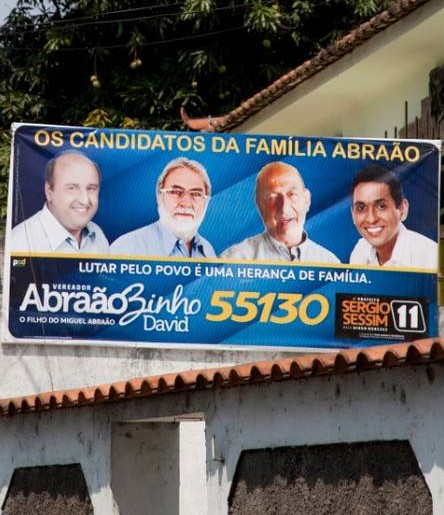
\includegraphics[width=.6\textwidth, height=8cm]{images/bicho08.jpg}
%  \caption{Political advertising for Abraãozinho David (right), nephew of the \emph{jogo do bicho} banker Aniz Abraão David (third from left to right). The banner reads: `The Candidates of the Abraão Family: Fighting for the People is a Family Heritage'. Source: \citet{extra2012aniz}.}
%  \label{fig:aniz}
% \end{figure}

The votes from poor communities are instrumental for aspiring politicians. Brazil has an enforced compulsory voting system; therefore, turnout rates tend to be higher than in other democracies. Consequently, votes have high marginal utility for politicians. As elections may be decided by a small difference, the \emph{bicheiros}' clientelistic ties guarantee a minimum number of votes that politicians can rely upon on election day. Nonetheless, the patronage subverts the preferences of the public and, as such, the democratic process per se. Individuals may be punished if the candidate does not receive the expected number of votes, and are often compelled to vote for politicians that have only loose connections with their communities. Therefore, although voters have the right to choose their representatives, in practice the suffrage is limited for a share of Brazil’s lower classes.

Finally, the \emph{jogo do bicho} patronage highlights a crucial social dilemma within the Brazilian public law. Even though federal judges have prosecuted \emph{bicheiros}, politicians and police forces have no incentives to enforce the punishment. Although Brazilian judges enjoy job stability, the latter groups constantly require local-level support from the \emph{bicheiros}. Politicians and police officers may have accurate information on \emph{jogo do bicho} operations and \emph{bicheiros}' whereabouts, but the federal government cannot rely upon their cooperation. That can be one of the reasons why even after many attempts to arrest \emph{bicheiros}, there has been little progress in that regard in Brazil's latest democratic period (1985--present).


\section{Concluding Remarks}
\label{sec:conclusion3}

Past research has shown that criminal organisations face considerable challenges to elicit cooperation from their members and establish close ties with the population \citep[e.g.][]{gambetta1996sicilian,skarbek2011governance,skarbek2012prison,varese2001russian,varese2011mafias}. Yet, the \textit{jogo do bicho} offers a convincing example that it is possible for an illegal syndicate to operate with low levels of violence for more than a hundred years. \textit{Bicheiros} employ a number of strategies to obtain reliable information from their subordinates while offering club goods and other selected benefits to workers. Furthermore, by investing in the Carnival parade \textit{bicheiros} have been able to gather popular and government support. Poor communities have associated with the \textit{bicheiros} to receive welfare provision, whereas politicians have collaborated with them to reap the financial and electoral benefits the \textit{jogo do bicho}'s networks can provide.
Past research has shown that criminal organisations face considerable challenges to elicit cooperation from their members and establish close ties with the population \citep[e.g.][]{gambetta1996sicilian,skarbek2011governance,skarbek2012prison,varese2001russian,varese2011mafias}. Yet, the \textit{jogo do bicho} offers a convincing example that it is possible for an illegal syndicate to operate with low levels of violence for more than a hundred years. \textit{Bicheiros} employ a number of strategies to obtain reliable information from their subordinates while offering club goods and other selected benefits to workers. Furthermore, by investing in the Carnival parade \textit{bicheiros} have been able to gather popular and government support. Poor communities have associated with the \textit{bicheiros} to receive welfare provision, whereas politicians have collaborated with them to reap the financial and electoral benefits the \textit{jogo do bicho}'s networks can provide.

Nevertheless, the \textit{jogo do bicho} has also created negative externalities. Violence is used to punish defectors and to constrain competitors. The clientelistic relationship that \textit{bicheiros} have with local politicians have lead to sub-optimal outcomes, such as predatory political campaigning, distortions in electoral representation, and impunity for human rights violations. These negative externalities have long-term effects and still impact the Brazilian public sphere.

Although the \textit{jogo do bicho} has received an increasing attention from scholars, much of its inner workings remain poorly understood. First, the relationship between \textit{bicheiros} and drug dealers is a topic that deserves attention. Brazil has become one of the world's largest consumers of illicit drugs and South America's principal drug trafficking transit route \citep{miraglia2015drugs,misse2011crime}. The question whether \textit{bicheiros} collaborated or opposed the emergent drug dealing business is still unclear. Second, the extent to which \textit{bicheiros} use other businesses, such as hotels or factories, to laundry money has been mentioned by members of the Brazilian judiciary \citep{globo2012bicheiro,globo2015cacaniquel}; however, there is no reliable estimate on its size. Lastly, more research is required to clarify how \textit{bicheiros} from different parts of Brazil coordinate their activities and prevent large-scale conflicts. Cases studies are usually focused on Rio de Janeiro's \textit{bicheiros}, but scholars would benefit from comparative analyses with a larger number of states. This is an important step to elucidate how \textit{bicheiros} continue to influence politics and the public across Brazil.

\newpage
\bibliography{bibliography.bib}
\bibliographystyle{apalike}
\end{document}

